\chapter{Metode}

\section{Razvojno okolje MATLAB}
Ves razvoj je potekal v programskem okolju MATLAB. Ta poleg samega programskega jezika vsebuje velik nabor že implementiranh funkcij, napredne aplikacije za strojno učenje in knjžnice ki omogočajo povezave z laboratorjskimi napravami. V njem sta ustvarjeni funkciji za računanje matrik Grangerjevega indexa vzročnosti
in matrik Kompleksnega Pearsonov korelacijskega koeficienta, prav tako so v njem ustvarjene nevronske mreže in uporabljeno je za ostale klasifikatorje in funkcijo za zajemanje podatkov iz naprave Cognionics Quick-20 ter funkcijo ki v realnem času razpoznava gibanje.
\begin{figure}[h!]
    \begin{center}
    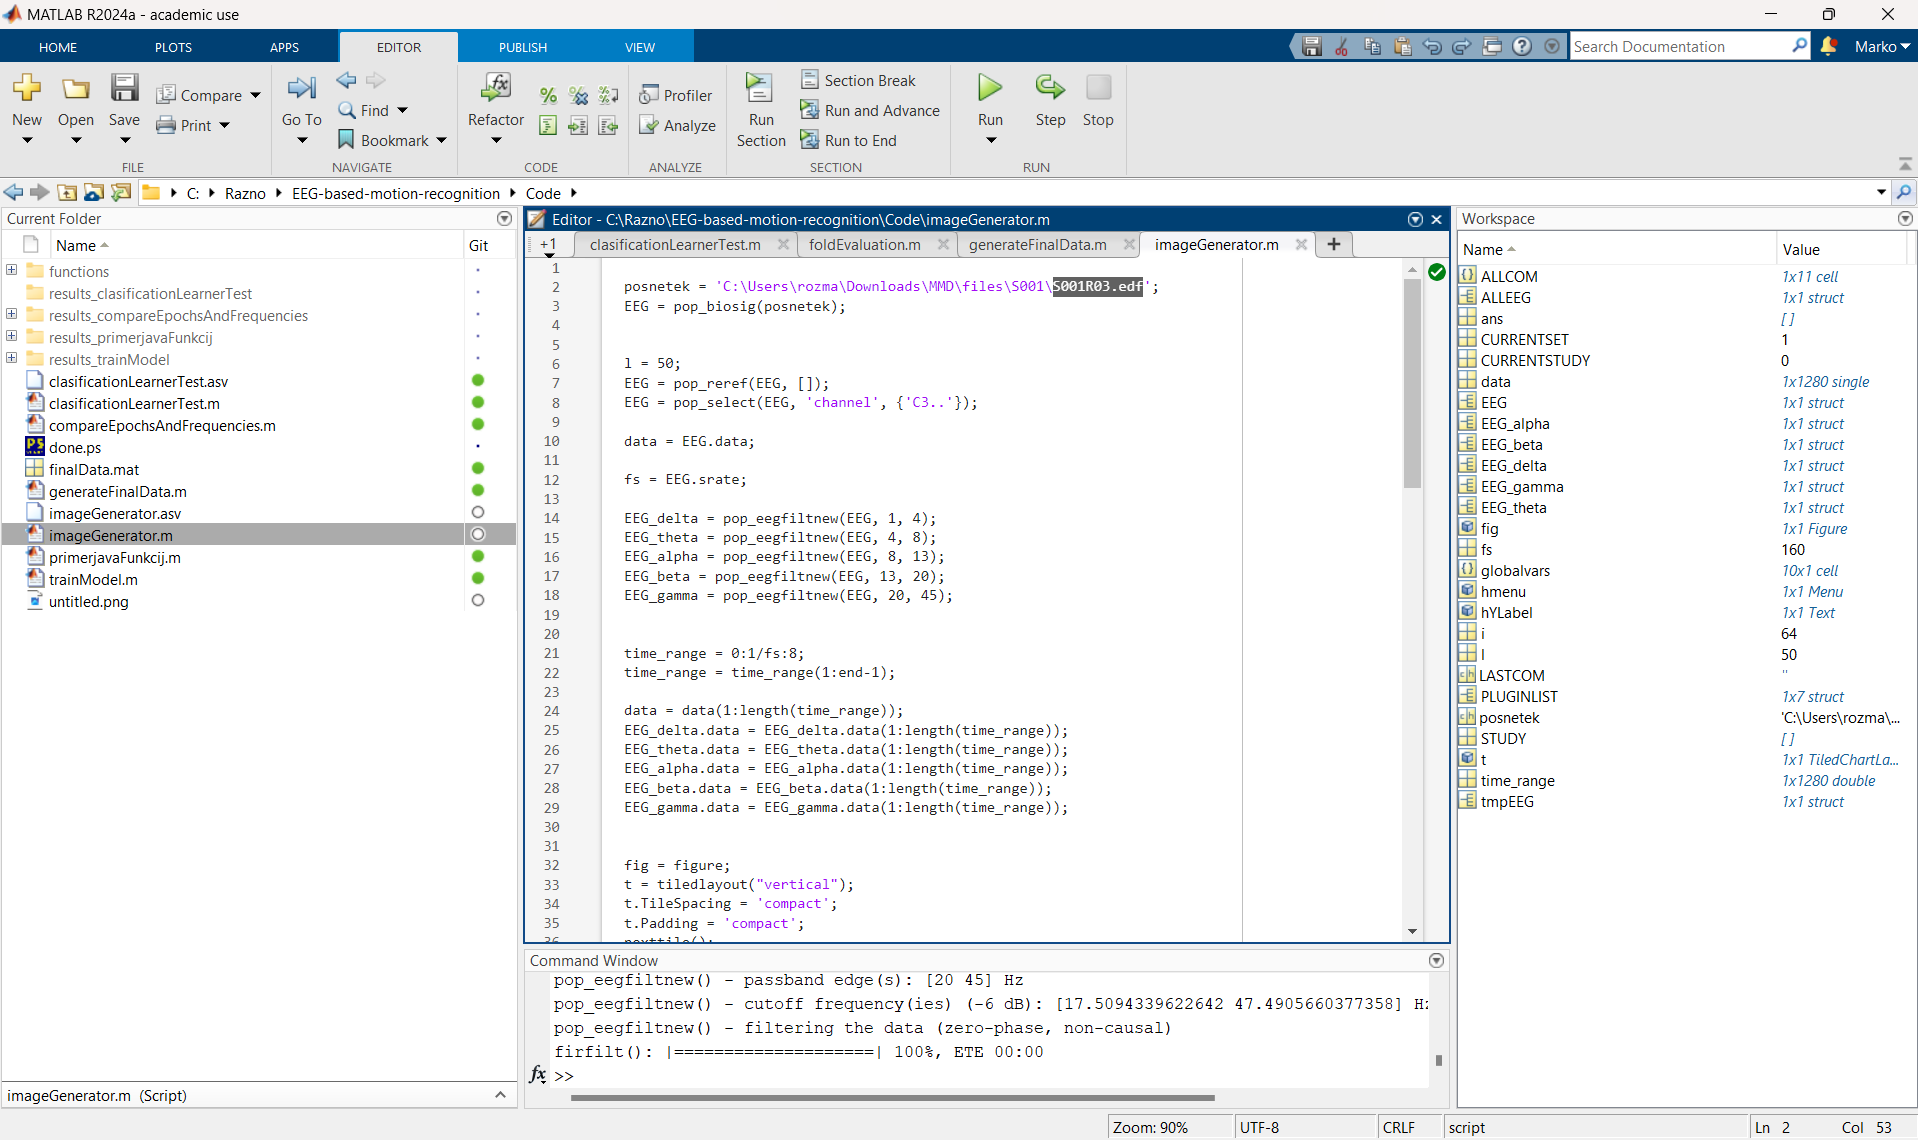
\includegraphics[width=1\linewidth]{slike/Matlab.png}
    \end{center}
    \caption{Programsko okolje MATLAB. Od leve proti desni: podokno z datotekami, podokno s kodo, podokno s spremenljivkami. Zgoraj zavihki za orodjarno, aplikacije in prikaz podatkov.}
    \end{figure}
    
\subsection{EEGLAB}
EEGLAB je interaktivna matlab orodjarna, za procesiranje in obdelavo elektrofizioloških podatkov. Omogoča rereferenciranje EEG signalov, izbiro določenih elektrod, deljenje podatkov na epohe glede na dogodke in filtriranje frekvenc. Omogoča interakcijo preko uporabniškega vmesnika. Vse akcije v vmesniku se prevedejo v ukaze ki jih lahko uporabimo v svoji kodi. Pri izdelavi naloge smo največ uporabljali funkcije branja .edf datotek, filtriranja frekvenc signalov in deljanja posnetkov na manjše dele.\cite{noauthor_eeglab_nodate}
\begin{figure}[h!]
    \begin{center}
    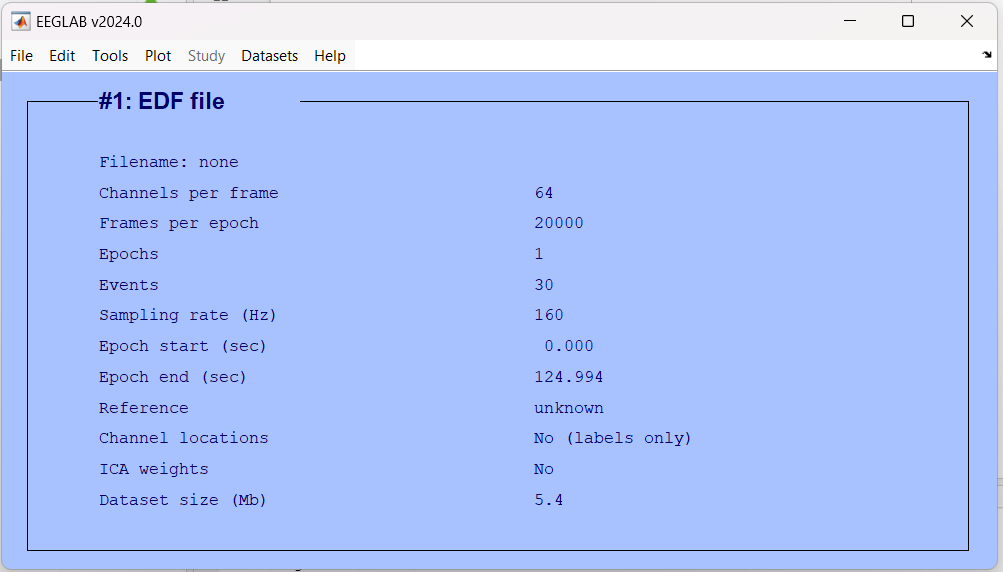
\includegraphics[width=1\linewidth]{slike/EEGLAB.png}
    \end{center}
    \caption{Orodjarna eeglab. Zgoraj zavihki za delo z datotekami, urejanje, orodja, prikaz podatkov, delo z zbirkami podatkov in pomoč. Naložen podatkovni niz dolžine 124 sekund z 30 dogodki.}
    \end{figure}

\subsection{Lab streaming layer}
Lab streaming layer je odprtokodna vmesna programska oprema ki omogoča pošiljanje, prejemanje, sinhronizacijo in snemanje tokov podatkov. Omogoča enostavno povezovanje EEG naprave z programsko opremo MATLAB. Knjižnjico je potrebno prenesti in nato zgraditi na svojem računalniku.  \cite{noauthor_lsl-website_nodate}

\subsection{Classification learner}
Classification learner je aplikacija v okolju MATLAB za enostavno klasifikacijo podatkov. Podpira različne metode klasifikacije, prečno preverjanje in uporabo različnih podatkov za gradnjo in testiranje modela. Aplikacija podpira klasifikacijo podatkov iz dvo dimenzionalnih matrik kjer vrstice ali stolpci predstavljajo spremenjlivke. Oznake podatkov lahko podamo kot določeno vrstico ali stolpec matrike ali v ločeni spremenljivki. Zaradi omejitev aplikacije smo pred klasifikacijo matrike povezljivosti prevorili v vektorje in te združili v matriko podatkov. Z aplikacijo smo lahko hitro ocenili uspešnost računanja matrik povezljivosti in primerjali delovanje različnih klasifikatorjev v primerjavi z našo nevronsko mrežo.
\begin{figure}[h!]
    \begin{center}
    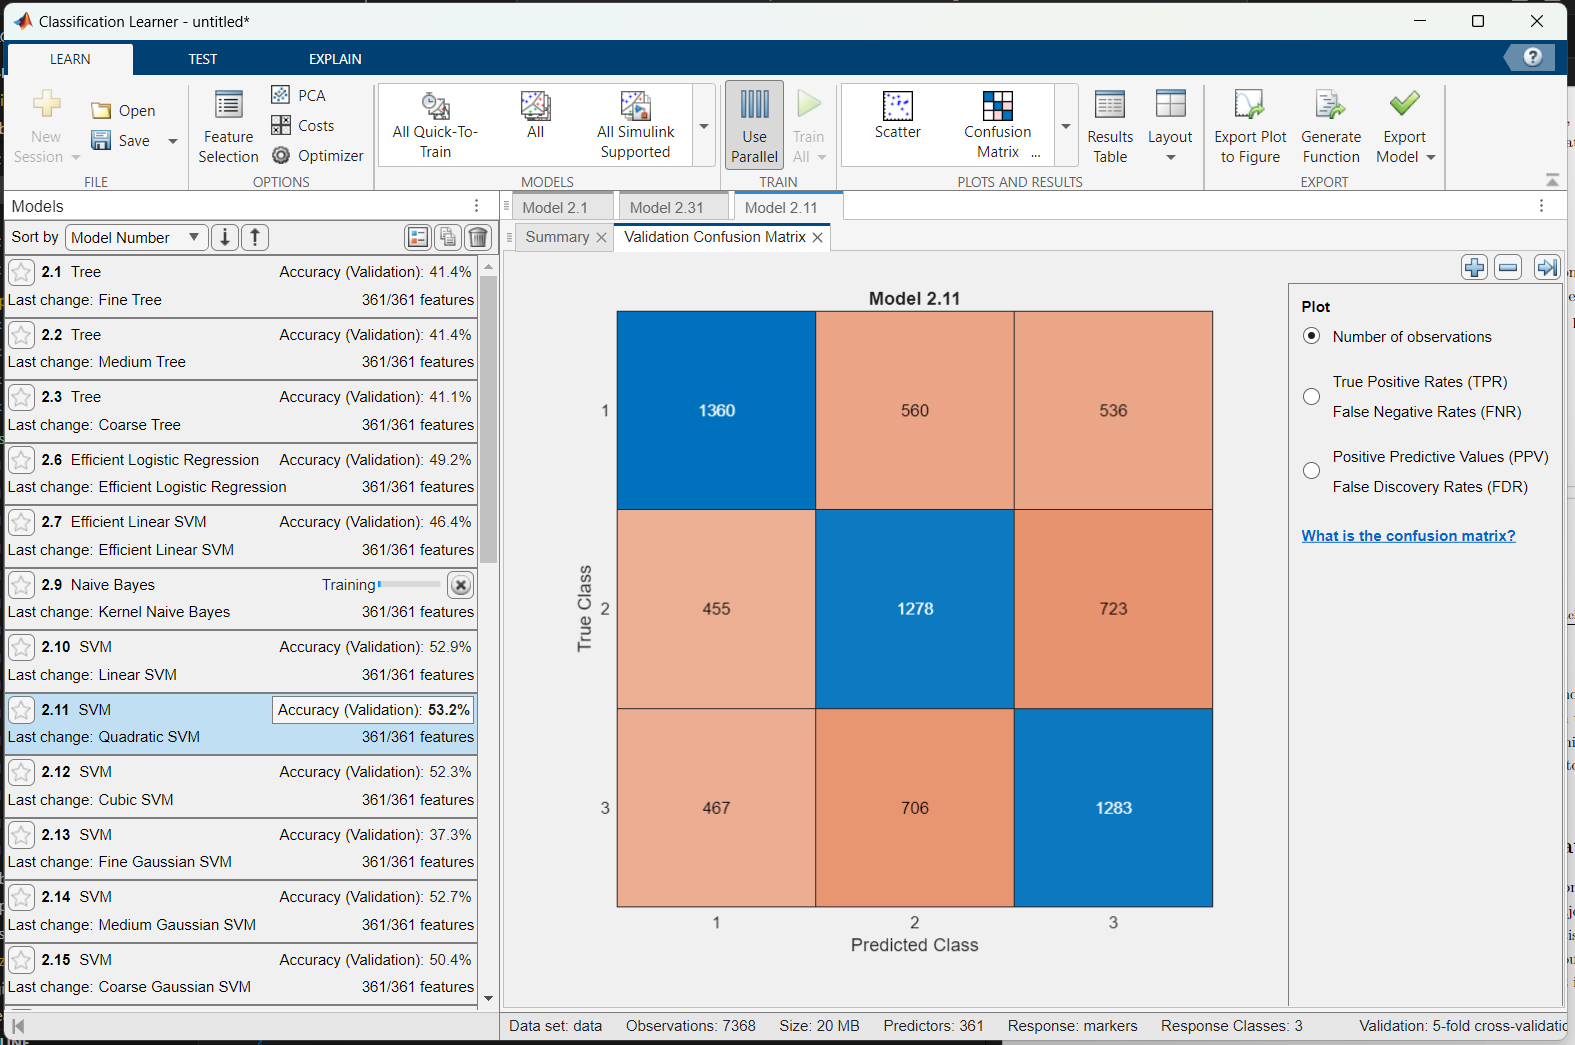
\includegraphics[width=1\linewidth]{slike/ClasificationLearner.png}
    \end{center}
    \caption{Aplikacija classification learner. Na levi strani podokno z različnimi metodami klasifikacije, na sredini prikaz podrobnosti izbrane metode. Zgoraj zavihki za učenje, testiranje in razlago. }
    \end{figure}

\section{EEG Motor Movement/Imagery Dataset}
EEG Motor Movement/Imagery Dataset(MMID) je prosto dostopna zbirka več kot 1500 eno in dve minutnih posnetkov 109 prostovoljcev. Zbirka za vsakega prostovoljca vsebuje dva izhodiščna posnetka in po tri posnetke opravljajanja štiri različnh nalog: stiskanje in sproščanje leve ali desne pesti(naloga 1), namišljeno stiskanje in sproščanje leve ali desne pesti(naloga 2), stiskanje in sproščanje obeh pesti ali obeh stopal(naloga 3), namišljeno stiskanje in sproščanje obeh pesti ali obeh stopal(naloga 4). Za nas relevantni so posnetki serij 3, 7 in 11 v katerih prostovoljci opravljajo prvo nalogo. Posnetki so shranjeni v formatu EDF+ ki vsebuje posnetke EEG in oznake dogodkov. Snemanje je bilo opravljeno z sistemom BCI2000 z 64 elektrodami postavljenimi po mednarodnem sistemu 10-10 brez elektrod Nz, F9, F10, FT9, FT10, A1, A2, TP9, TP10, P9, in P10.\cite{schalk_eeg_2009,schalk_bci2000_2004}

\begin{table}[h]
\centering
\begin{tabular}{|c|c|l|}

\hline
Številka serije & Naloga &Opis naloge \\
\hline
1 & izhodišče & odpte oči  \\
\hline
2 & izhodišče & zaprte oči  \\
\hline
3 & naloga 1 & stiskanje in sproščanje leve ali desne pesti \\
\hline
4 & naloga 2 &namišljeno stiskanje in sproščanje leve ali desne pesti  \\
\hline
5 & naloga 3 &stiskanje in sproščanje obeh pesti ali obeh stopal \\
\hline
6 & naloga 4 &namišljeno stiskanje in sproščanje obeh pesti ali obeh stopal  \\
\hline
7 & naloga 1 &stiskanje in sproščanje leve ali desne pesti \\
\hline
8 & naloga 2 &namišljeno stiskanje in sproščanje leve ali desne pesti  \\
\hline
9 & naloga 3 &stiskanje in sproščanje obeh pesti ali obeh stopal \\
\hline
10 & naloga 4 &namišljeno stiskanje in sproščanje obeh pesti ali obeh stopal  \\
\hline
11 & naloga 1 &stiskanje in sproščanje leve ali desne pesti \\
\hline
12 &naloga 2 &namišljeno stiskanje in sproščanje leve ali desne pesti  \\
\hline
13 & naloga 3 &stiskanje in sproščanje obeh pesti ali obeh stopal \\
\hline
14 & naloga 4 &namišljeno stiskanje in sproščanje obeh pesti ali obeh stopal  \\

\hline
\end{tabular}
\caption{Naloge in opisi nalog, ki jih prostovoljci opravljajo v posnetkih zbirke podtakov MMID.}
\end{table}

\begin{figure}[h!]
    \begin{center}
    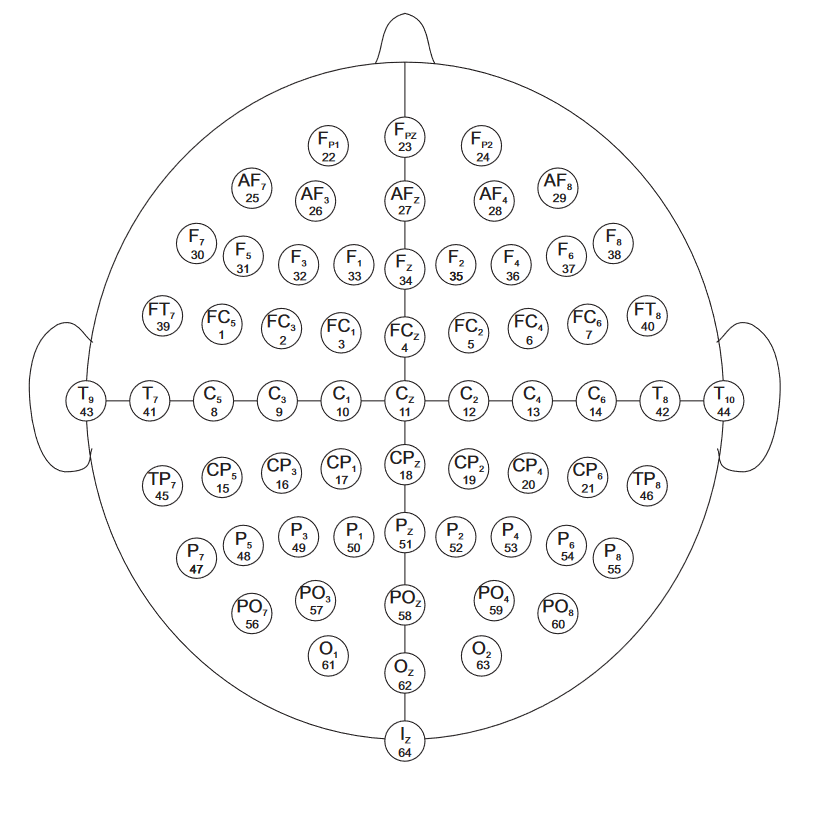
\includegraphics[width=1\linewidth]{slike/64electrodeSystem.png}
    \end{center}
    \caption{Postavitev elektrod po mednarodnem sistemu 10-10 brez elektrod Nz, F9, F10, FT9, FT10, A1, A2, TP9, TP10, P9, in P10, ki je blia uporabljena za snemanje zbirke MMID.}
    \end{figure}
\section{Metode povezljivosti}
\subsection{Grangerjev index vzročnosti}
Grangerjev index vzročnosti je statistična metoda za preverjanje ali ena časovna vrsta nosi informacije o drugi. Metoda je bila razvita v šestdesedih letih devetnajstega stoletja za uporabo ekonomiji.

Za dve časovni vrsti $X_1$ in $X_2$, in $p$ kot število prejšnjih vrednosti ki jih upoštevamo pri računanju, lahko izračunamo $E_1$ in $E_1$ ki so napake pri predvidevanju naslednje vrednosti v vrsti $X_1$. V kolikor je varianca vrednosti $E_2$ manjša kot varianca vrednosti $E_1$ lahko predvidevamo da časovna vrsta $X_2$ nosi informacije o časovni vrsti $X_1$
\begin{align*}
X_1(t) &= \sum_{j=1}^{p} A_{1,j} X_1(t-j) + E_1(t)\\
X_1(t) &= \sum_{j=1}^{p} A_{2,j} X_1(t-j) + \sum_{j=1}^{p} A_{3,j} X_2(t-j) + E_2(t)
\end{align*}


\textcolor{red}{Mogoče razlaga kaj so A-ji. Ali je pravilno razloženo?}

\cite{seth_granger_2007}

\subsection{Kompleksni Pearsonov korelacijski koeficient}
Pearsonov korelacijski koeficient je najpogosteje uporabljen linearni korelacijski koeficient. Zanj smo se odločili saj v članku  \citetitle{sverko_complex_2022} avtorji pokažejo da vsebuje informacije PLI in wPLI ki sta dve najbolj pogosto uporabljeni metodi povezljivosti. V praksi nam pove, v kakšni meri sta fazi dveh signalov linearno povezani.

Ker želimo opazovati faze EEG signala, ga potrebujemo pretvoriti v analitični signal ki vsebuje informacijo o fazi. Zaradi sledeče transformacijo, ki je definirana samo na ozkih frekvenčnih pasovih potrebujemo signale EEG predhodno filtrirati. Analitični signal $X_a$ kjer $HT(X(t))$ označuje hilbertovo transformacijo signala $X$.
\begin{align*}
    X_a(t) = X(t) + i \cdot HT(X(t))
\end{align*}

Za računanje Kompleksnega Pearsonovega korelacijskega koeficienta v našem primer lahko uporabimo naslednjo enačbo kjer sta $X_1$ in $X_2$ analitična signal dolžine $N$. $\overline{X_2(n)}$ pa konjugirana vrednost $X_2(n)$
\begin{align*}
r(X_1, X_2) &= \frac{\sum\limits_{n=1}^{N}(X_1(n) \cdot \overline{X_2(n)})}{\sqrt{\sum\limits_{n=1}^{N} |X_1(n)|^2} \cdot \sqrt{\sum\limits_{n=1}^{N} |X_2(n)|^2}}
\end{align*}
\cite{sverko_complex_2022} 

\section{Klasifikacija}
Želeli smo preizkusiti kako uspešno bi klasifikacija delovala na podatkih zbirke in kako uspešno bi delovala na naših podatkih, zato smo klasifikacijo izvajali dvakrat. Enkrat na podatkih zbirke in enkrat na naših podatkih. Ker nevronska mreža za učenje potrebuje več podatkov kot jih lahko zagotovimo iz naših posnetkov smo jo za namene klasifikacije naših posnetkov naučili na podatkih MMID in nato dodatno naučili na naših podatkih. 

\subsection{Classification learner}
Na matrikah povezljivosti pridobljenih iz podatkov zbirke in naših posnetkov smo izvedli več različnih klasifikacije in sicer: odločitvena drevesa, metodo k najbližjih sosedov (k-NN), logistično regresijo, podporne vektorske stroje (SVM) in nevronske mreže.


\subsection{Nevronska mreža}
Nevronska mreža je sestavljena iz vhodne plasti za slike dimenzij 19x19x1, polno povezane plasti s 100 nevroni, Leaky ReLU plasti, dropout plasti z 50\% verjetnostjo opustitve nevronov, polno povezane plasti z 10 nevroni, GELU plasti, dropout plasti z 50\% verjetnostjo opustitve nevronov, polno povezane plasti s tremi nevroni in Softmax plasti. 
\begin{figure}[h!]
\begin{center}
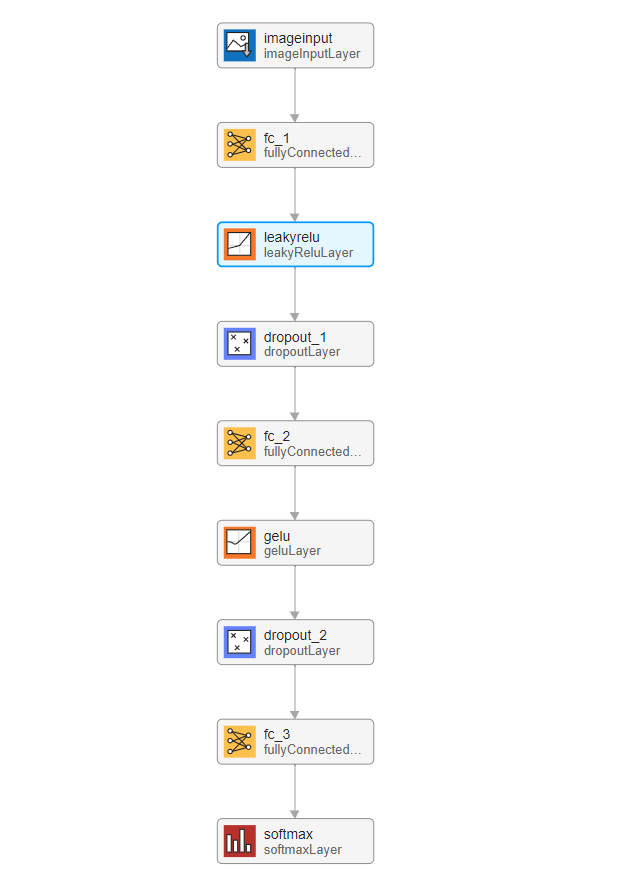
\includegraphics[width=0.8\linewidth]{slike/Neural network.png}
\end{center}
\caption{Prikaz plasti nevronske mreže v MATLAB alikaciji Deep Network Designer. Od zgoraj navzdol: plast za slike, polno povezana, Leaky ReLU, dropout, polno povezana, GELU, dropout, polno povezana in Softmax.}
\end{figure}






